\documentclass{article}
\usepackage[utf8]{inputenc}
\usepackage[margin=2cm]{geometry}
\usepackage{fullpage,enumitem,amssymb,amsmath,xcolor,cancel,gensymb,hyperref,graphicx}
\usepackage[brazilian]{babel}
\usepackage{indentfirst}
\usepackage{graphicx}
\usepackage{caption}
\usepackage{tabularx}
\usepackage{array}
\usepackage{float}
\usepackage{booktabs, multirow}

\begin{document}
\begin{center}
    \textbf{\LARGE MAP2212 - Laboratório de Computação e Simulação}\\
    \vspace{0.3cm}
    \textbf{\Large Relatório - EP03}\\
    \vspace{0.3cm}
    \large{Vítor Garcia Comissoli - 11810411}
\end{center}

\section{Introdução}

    O objetivo desse EP é a refacção do EP02 só que utilizando geradores de números quasi-random ao invés de geradores de números pseudo-aleatórios nos quatro métodos de Monte Carlo (\textbf{Crude}, \textbf{Hit or Miss}, \textbf{Control Variate} e \textbf{Importance Sampling}).\\
    
    Além disso, deve-se comparar a diferenças nos valores obtidos para \textbf{n} nos quatro métodos, para que a estimativa de $\gamma$ obtida tenha um erro de, no máximo, 0.05\% de $\gamma$, com 95\% de confiança, ou seja, que fique dento do Intervalo de Confiança $[\gamma\cdot(1 - 0.0005),\gamma\cdot(1 + 0.0005)]$ com $\alpha=0.95$.\\
    
    Geradores quasi-random são aqueles que, ao contrário dos pseudo-aleatórios, seguem um certo padrão sistemático durante a geração dos pontos, ou seja, são geradores que geram números pouco discrepantes entre sí, o que costuma levar a um melhor desempenho quando utilizados em casos como o desse EP (estimações que tendem a um valor específico, nesse caso que tendem a $\gamma$).\\
    
    Vale ressaltar também que, neste EP, deve-se tratar o valor da integral $\gamma$ como desconhecido, então todos os testes devem ser realizadas com um estimador qualquer para $\gamma$ ($\hat{\gamma}$).
    
\section{Discussão Teórica}
    
    Como esse EP é um complemento do EP02, a maior parte da discussão teórica  seria a mesma, por isso optei por não me repetir. Em suma, temos que os valores de \textbf{n} calculados para os quatro métodos no caso pseudo-aleatório são:\\
    \\
    Para \textbf{Crude}, $n = 4502884$\\
    Para \textbf{Hit or Miss}, $n = 14853316$\\
    Para \textbf{Control Variate}, $n =  100000$\\ 
    Por fim, para \textbf{Importance Sampling}, $n = 3541924$\\
    
    Como o objetivo desse EP é a subistituição dos geradores númericos pseudo-aleatórios por geradores quasi-random, haverá uma discrepância nos valores de \textbf{n} necessários para que se atinja a precisão de $\gamma\cdot(1 + 0.0005)]$ com $\alpha=0.95$. Sabendo disso, Devemos encontrar os novos valores de \textbf{n} para que possamos analisar a diferença entre cada um dos valores de \textbf{n} para cada um dos métodos.\\
    
    Os novos valores de n foram encontrados de forma experimental, ou seja, os valores de \textb{n} de EP02 foram sendo gradativamente reduzidos (cada método foi individualmente observado e testado para que se encontra-se o valor de n específico para o mesmo.) até que não se enquadrassem mais no intervalo solicitado, decidindo-se assim que o novo valor de \textb{n} seja o menor valor de \textb{n} que mostrou-se coerente a precisão solicitada em cada um dos métodos.\\
    
    Os testes de intervalo foram realizados por meio de uma função main() que chama as funções de cada um dos métodos \textbf{n} vezes e retorna a razão das estimativas para $\gamma$ que se encontram dentro do intevalo de confiança sobre o número total de estimativas realizadas, sendo que o intervalo utilizado pela mesma foi obtido através do uso de $\hat{\gamma} = 0.74391$ (proveniente da função control\_variates() para um n = 1000000).\\
    \\
    Disso, chegamos em quatro novos valores para \textb{n}, um para cada método, sendo eles:\\
    \\
    Para \textbf{Crude}, novo $n = 700000$\\
    Para \textbf{Hit or Miss}, novo $n = 6000000$\\
    Para \textbf{Control Variate}, novo $n =  750$\\ 
    Por fim, para \textbf{Importance Sampling}, novo $n = 150000$\\

\section{Discussão do Código}

Os prints abaixo do código estão comentados linha por linha, explicitando todos os processos tomados.

    \begin{figure}[H]
        \centering
        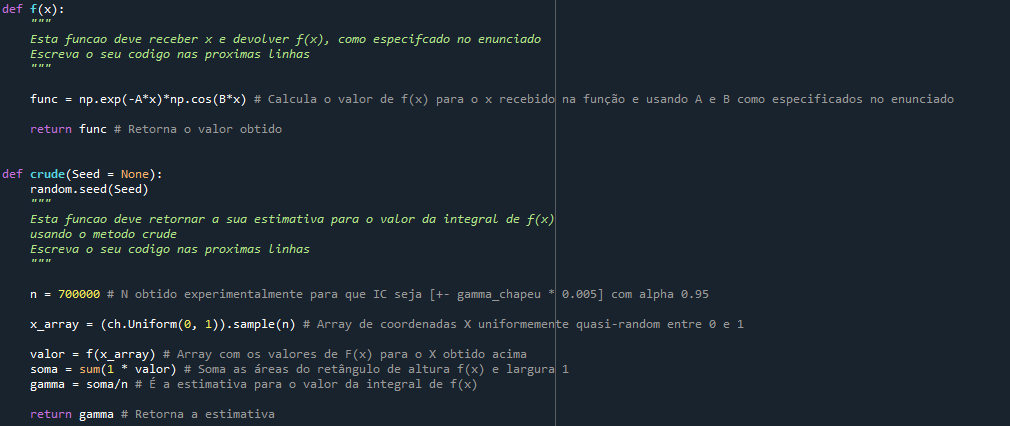
\includegraphics[width= 1 \textwidth]{Código f(x) e crude.png}
        \caption{Código e comentários das funções f(x) e Crude}
        \label{fig:grafico}
    \end{figure}
    
    \begin{figure}[H]
        \centering
        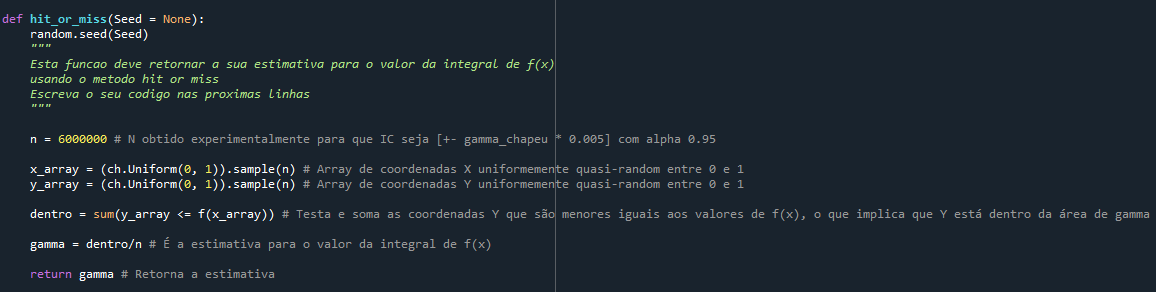
\includegraphics[width= 1 \textwidth]{Código hit or miss.png}
        \caption{Código e comentários da função Hit or Miss}
        \label{fig:grafico}
    \end{figure}

    \begin{figure}[H]
        \centering
        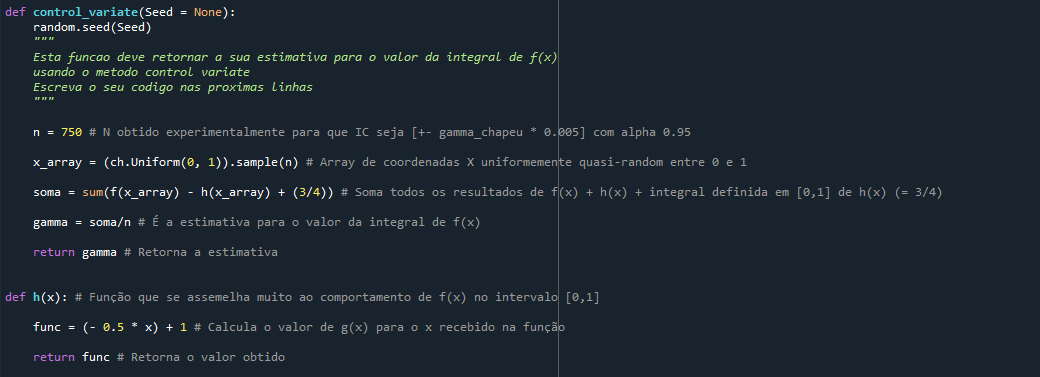
\includegraphics[width= 1 \textwidth]{Código control variate.png}
        \caption{Código e comentários da função Control Variate}
        \label{fig:grafico}
    \end{figure}
    
    \begin{figure}[H]
        \centering
        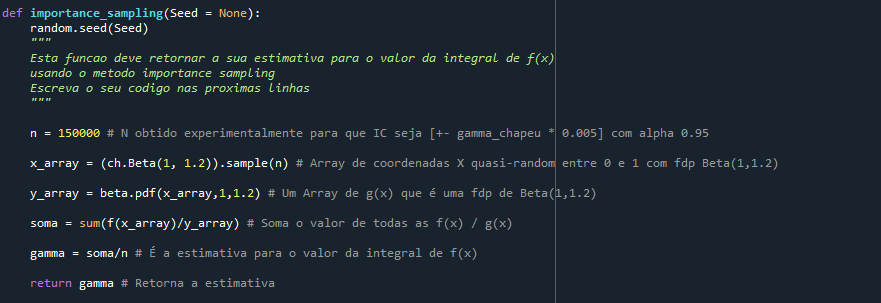
\includegraphics[width= 1 \textwidth]{Código importance sampling.png}
        \caption{Código e comentários da função Importance Sampling}
        \label{fig:grafico}
    \end{figure}

Além disso, vale ressaltar que foi-se utilizada a biblioteca \textbf{chaospy} para a obtenção das coordenadas quasi-random nos quatro métodos.

\section{Resultado}

O teste dos resultados foi realizado pela criação de uma função main() que chama as funções dos quatro métodos \textbf{n} vezes e imprime a razão das estimativas para $\gamma$ que se encontram dentro do intevalo de confiança (intervalo esse obtido através do uso de $\hat{\gamma} = 0.74391$, proveniente da função control\_variates() para um n = 1000000) sobre o número total de estimativas realizadas, além de apresentar a média amostral dessas \textbf{n} saídas e o tempo total gasto.\\
\\
Para o método Crude, cujo valor de $\textbf{n}$ era $4502884$ para geradores pseudo-aleatórios (EP02), obteve-se experimentalmente para geradores quasi-random $n = 700000$, o que demonstra a necessidade de um n aproximadamente 6.5 vezes menor para que se atinja uma precisão semelhante. Na main(), para $n = 1000$, essa razão foi de $0.964$, com média $\mu = 0.74391$. O tempo gasto para um loop de $n = 1000$ foi de, aproximadamente, $110.77$ segundos ($1.85$ min).\\
\\
Já para o método Hit or Miss, cujo valor de $\textbf{n}$ era $14853316$ para geradores pseudo-aleatórios (EP02), obteve-se experimentalmente para geradores quasi-random $n = 6000000$, o que demonstra a necessidade de um n aproximadamente 2.5 vezes menor para que se atinja uma precisão semelhante. Na main(), para $n = 100$, essa razão foi de $0.97$, com média $\mu = 0.74391$. O tempo gasto para um loop de $n = 100$ foi de, aproximadamente, $1645.25$ segundos ($27.42$ min).\\
\\
Para o método Control Variate, cujo valor de $\textbf{n}$ era $100000$ para geradores pseudo-aleatórios (EP02), obteve-se experimentalmente para geradores quasi-random $n = 750$, o que demonstra a necessidade de um n aproximadamente 133 vezes menor para que se atinja uma precisão semelhante. Na main(), para $n = 10000$, essa razão foi de $0.9564$, com média $\mu = 0.74392$. O tempo gasto para um loop de $n = 10000$ foi de, aproximadamente, $11.80$ segundos ($0.20$ min).\\
\\
Por fim, para o método Important Sampling, cujo valor de $\textbf{n}$ era $3541924$ para geradores pseudo-aleatórios (EP02), obteve-se experimentalmente para geradores quasi-random $n = 150000$, o que demonstra a necessidade de um n aproximadamente 23.6 vezes menor para que se atinja uma precisão semelhante. Na main(), para $n = 1000$, essa razão foi de $0.972$, com média $\mu = 0.74392$. O tempo gasto para um loop de $n = 1000$ foi de, aproximadamente, $467.78$ segundos ($7.80$ min).\\
\\
Todos os valores apresentados acima mostram-se coerentes aos parâmetros de acurácia $\alpha = 0.95$ e $\epsilon = \gamma \cdot0.0005$, estipulados pelo enunciado do EP. \\
\\
Com isso podemos concluir que o resultado obtido foi dentro do esperado.

\section{Conclusão}

Como já dito previamente, todos o métodos se mostraram coerentes aos parâmetros de acurácia de $\alpha = 0.95$ e $\epsilon = \gamma \cdot0.0005$. Contudo, existem outros fatores que podem ser analisados.\\
\\
Analisando quanto a performance computacional, não faz sentido comparar os métodos do EP03 com os mesmos no EP02, visto que para esse EP otimizei todos os quatro métodos por meio da vetorização e uso de arrays, enquanto o anterior se utiliza-va somente de "for \_ in range(\_)", o que faz com que todos os métodos desse EP se mostrem mais rápidos que suas contrapartidas no EP anterior. Faz sentido porém, comparar a performance de cada um dos quatro métodos desse EP entre sí. Temos que o método de Hit or Miss se mostrou muito lento e custoso quando comparado com os outros 3 métodos, seguido pelo método Importance Sampling, o método Crude e, por fim, o método Control Variate, que se mostrou o mais eficiente.\\
\\
Por fim, quanto ao tamanho do \textbf{n} encontrado, pode-se perceber que todos os valores de n para os métodos do EP03 foram menores que seus respectivos n obtidos no EP02, o que mostra que o uso de geradores de números quasi-random mostra-se mais eficaz nesse tipo de aplicação que o uso de geradores pseudo-aleatórios comúns, já que os quasi-random convergiram mais rapidamente para o valor de $\gamma$. Quando comparamos o tamanho dos valores de n entre os modelos do próprio EP03, temos que o método Hit or Miss necessitou do maior valor de n, seguido pelo método Crude, pelo método Importance Sampling e, por fim, pelo método Control Variate, que foi o que utilizou o menor valor de n dentre os quatro.

\end{document}